\documentclass[10pt, aspectratio=169, handout]{beamer}
\usefonttheme{professionalfonts}

\mode<presentation>{
  \usetheme{Berkeley}
  \usecolortheme{beaver}
  \usefonttheme{default}
  \setbeamertemplate{navigation symbols}{}
  \setbeamertemplate{caption}[numbered]
}

\setbeamertemplate{footline}{%
  \leavevmode%
  \hbox{%
    \begin{beamercolorbox}[wd=.85\paperwidth,ht=2.5ex,dp=1ex,left]{author in head/foot}%
      \usebeamerfont{author in head/foot}Digital Signal Processing, Fall 2025%
    \end{beamercolorbox}%
    \begin{beamercolorbox}[wd=.15\paperwidth,ht=2.5ex,dp=1ex,right]{date in head/foot}%
      \hspace*{0.5em}\insertframenumber{} / \inserttotalframenumber\hspace*{0.5em}%
    \end{beamercolorbox}%
  }%
  \vskip0pt%
}

\usepackage[english]{babel}
\usepackage[utf8]{inputenc}

\usepackage{tikz}
\usepackage{pgfplots}
\usepgfplotslibrary{groupplots}
\usetikzlibrary{calc, positioning, arrows.meta, backgrounds, pgfplots.fillbetween, pgfplots.groupplots, plotmarks}

\pgfplotsset{compat=newest}

\usepackage{array}
\usepackage{makecell}
\usepackage{verbatim}
\usepackage{graphicx}
\usepackage{amsfonts}
\usepackage{amsmath}
\usepackage{bm}
\usepackage{epstopdf}
\usepackage[absolute,overlay]{textpos}

\usepackage{hyperref}
\hypersetup{
    colorlinks=true,
    linkcolor=blue,
    filecolor=magenta,
    urlcolor=cyan,
}

\title[ECEN 463/863]{Sampling Rate Conversions: Downsampling}
\author{Maxx Seminario}
\institute{University of Nebraska-Lincoln}
\date{Fall 2025}

\begin{document}

\begin{frame}
  \titlepage
\end{frame}

\begin{frame}{Downsampling: Motivation}
\small
\textbf{Why downsample?}
\begin{itemize}
  \item Reduce computation, memory, bandwidth, and power.
  \item Match device/IO rate constraints (sensors, radios, codecs).
  \item Enable multirate algorithms, filter banks.
\end{itemize}

\vspace{0.2cm}
\textbf{Definition (Compressor / Downsampler):}
\[
x_d[n] = x[nM] = x_c(nMT) \quad \text{with} \quad T_d = MT
\]
Equivalent to sampling the bandlimited reconstruction \(x_c(t)\) with period \(T_d\).

\end{frame}

\begin{frame}{Downsampling: Aliasing Considerations}

\textbf{When is it alias-free?}
\begin{itemize}
  \item If \(X_c(j\Omega)=0\) for \(|\Omega|\ge \Omega_N\), then \(x_d[n]\) exactly represents \(x_c(t)\) if
  \[
  \frac{\pi}{T_d} = \frac{\pi}{MT} \ge \Omega_N \;\;\Longleftrightarrow\;\; \omega_N \le \frac{\pi}{M}.
  \]
  \item Interpretations:
    \begin{itemize}
      \item Original sampling rate is at least \(M\) times the Nyquist rate, or
      \item Prefilter to reduce bandwidth by factor \(M\) before downsampling (decimation).
    \end{itemize}
\end{itemize}

\vspace{0.2cm}
\textbf{Terminology:}
\begin{itemize}
  \item Compressor: just \(\downarrow M\) (rate reduction).
  \item Decimator: antialiasing lowpass + \(\downarrow M\).
\end{itemize}

\begin{center}
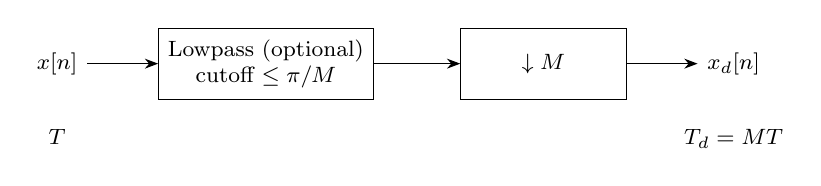
\begin{tikzpicture}[>=Stealth, node distance=0.8cm, auto, every node/.style={font=\footnotesize}]
  \tikzset{block/.style={draw, minimum width=2.1cm, minimum height=0.9cm, align=center}}
  \node (xn) {$x[n]$};
  \node[block, right=0.9cm of xn] (lpf) {Lowpass (optional)\\cutoff $\le \pi/M$};
  \node[block, right=1.1cm of lpf] (down) {$\downarrow M$};
  \node (xd) [right=0.9cm of down] {$x_d[n]$};

  \draw[->] (xn.east) -- (lpf.west);
  \draw[->] (lpf.east) -- (down.west);
  \draw[->] (down.east) -- (xd.west);

  \node[below=0.45cm of xn] {$T$};
  \node[below=0.45cm of xd] {$T_d=MT$};
\end{tikzpicture}
\end{center}
\end{frame}

\section{Frequency-Domain Analysis}

\begin{frame}{Frequency-Domain Analysis}
\small
\textbf{DTFT Relationship}:

DTFT of $x[n] = x_c(nT)$:
\[
X(e^{j\omega}) = \frac{1}{T}\sum_{k=-\infty}^{\infty} X_c\!\left(j\frac{\omega}{T} - j\frac{2\pi k}{T}\right)
\]

Downsampled sequence DTFT (with $T_d = MT$):
\[
X_d(e^{j\omega}) = \frac{1}{T_d}\sum_{r=-\infty}^{\infty} X_c\!\left(j\frac{\omega}{T_d} - j\frac{2\pi r}{T_d}\right)
\]

\textbf{Key Result -- Relationship Between DTFTs}:
\[
X_d(e^{j\omega}) = \frac{1}{M} \sum_{i=0}^{M-1} X\!\left(e^{j(\omega/M - 2\pi i/M)}\right)
\]

\textbf{Interpretation}:
\begin{itemize}
    \item \(X_d(e^{j\omega})\) is sum of \(M\) scaled, shifted copies of \(X(e^{j\omega})\).
    \item Frequency axis compressed by factor \(M\); shifts at \(2\pi i/M\).
    \item Overall amplitude scaling \(1/M\).
\end{itemize}
\end{frame}

\begin{frame}{Derivation of DTFT Relationship}
\small
Starting point (sampling with \(T_d = MT\)):
\[
X_d(e^{j\omega}) = \frac{1}{MT}\sum_{r=-\infty}^{\infty} X_c\!\left(j\frac{\omega}{MT} - j\frac{2\pi r}{MT}\right)
\]

Let \( r = i + kM\) with \( i = 0,1,\dots,M-1\):
\[
X_d(e^{j\omega}) = \frac{1}{MT}\sum_{i=0}^{M-1}\sum_{k=-\infty}^{\infty}
X_c\!\left(j\frac{\omega}{MT} - j\frac{2\pi (i + kM)}{MT}\right)
\]

Group terms:
\[
X_d(e^{j\omega}) = \frac{1}{M}\sum_{i=0}^{M-1}\frac{1}{T}\sum_{k=-\infty}^{\infty}
X_c\!\left(j\frac{\omega - 2\pi i}{MT} - j\frac{2\pi k}{T}\right)
\]

Recognize inner sum as \(X\big(e^{j(\omega/M - 2\pi i/M)}\big)\). Therefore:
\[
\boxed{X_d(e^{j\omega}) = \frac{1}{M} \sum_{i=0}^{M-1} X\!\left(e^{j(\omega/M - 2\pi i/M)}\right)}
\]
\end{frame}

\begin{frame}{Downsampling Example: $M=2$ (No Aliasing)}
\small
Setup: Original sampling rate is twice the minimum Nyquist rate; bandwidth fits after compression.

\begin{center}
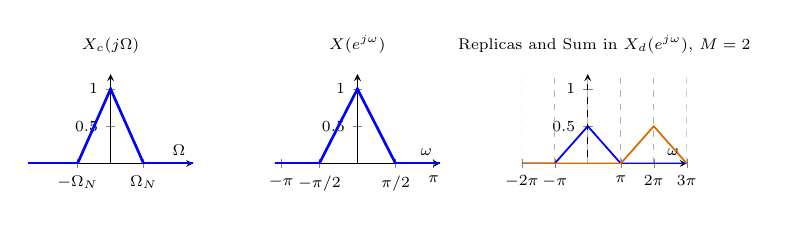
\begin{tikzpicture}[scale=0.8]
  \begin{groupplot}[
    group style={group size=3 by 1, horizontal sep=1.3cm},
    width=4.2cm,
    height=3cm,
    axis lines=middle,
    ymin=0, ymax=1.2,
    tick label style={font=\scriptsize},
    label style={font=\scriptsize},
    title style={font=\scriptsize}
  ]
  % --- Continuous-time spectrum (illustrative) ---
  \nextgroupplot[
    title={$X_c(j\Omega)$},
    xmin=-5, xmax=5,
    xtick={-2,0,2},
    xticklabels={$-\Omega_N$,$0$,$\Omega_N$},
    xlabel={$\Omega$}, ylabel={}
  ]
  \addplot[blue, very thick] coordinates {(-5,0) (-2,0) (0,1) (2,0) (5,0)};

  % --- DTFT of x[n] ---
  \nextgroupplot[
    title={$X(e^{j\omega})$},
    xmin=-3.4, xmax=3.4,
    xtick={-3.1416,-1.5708,0,1.5708,3.1416},
    xticklabels={$-\pi$,$-\pi/2$,$0$,$\pi/2$,$\pi$},
    xlabel={$\omega$}
  ]
  \addplot[blue, very thick] coordinates {(-3.4,0) (-1.5708,0) (0,1) (1.5708,0) (3.4,0)};

  % --- Downsampled: show replicas (i=0 and i=1) and their sum ---
  \nextgroupplot[
    title={Replicas and Sum in $X_d(e^{j\omega}),\,M=2$},
    xmin=-2*pi, xmax=3*pi,        % expanded so i=1 at 2π spans [π, 3π]
    ymin=0, ymax=1.2,
    xtick={-2*pi,-pi,0,pi,2*pi,3*pi},
    xticklabels={$-2\pi$,$-\pi$,$0$,$\pi$,$2\pi$,$3\pi$},
    xlabel={$\omega$}
  ]

  % Guides at key centers -2π, -π, 0, π, 2π, 3π
  \draw[gray!60, dashed] (axis cs:-2*pi,0) -- (axis cs:-2*pi,1.15);
  \draw[gray!60, dashed] (axis cs:-pi,0)   -- (axis cs:-pi,1.15);
  \draw[gray!60, dashed] (axis cs:0,0)     -- (axis cs:0,1.15);
  \draw[gray!60, dashed] (axis cs: pi,0)   -- (axis cs: pi,1.15);
  \draw[gray!60, dashed] (axis cs: 2*pi,0) -- (axis cs: 2*pi,1.15);
  \draw[gray!60, dashed] (axis cs: 3*pi,0) -- (axis cs: 3*pi,1.15);

  % Assume original bandedge ω_N = π/2 (safe for M=2), so compressed baseband half-width = π.

  % Replica i=0 (centered at 0): (1/2) * triangular shape with width 2π (half-width π)
  \addplot[blue, thick, domain=-2*pi:3*pi, samples=500]
    {(1/2.0) * max(0, 1 - abs(x)/(pi))};

  % Replica i=1 (shifted by 2π/M = π per copy index, but summed copies at multiples of 2π):
  % For M=2, the non-zero terms in the aliasing sum appear at multiples of 2π. Center this at 2π.
  % This triangle spans [π, 3π] with peak at 2π.
  \addplot[orange!85!black, thick, domain=-2*pi:3*pi, samples=500]
    {(1/2.0) * max(0, 1 - abs(x - 2*pi)/(pi))};

  \end{groupplot}
\end{tikzpicture}
\end{center}

Result: No aliasing because the compressed baseband fits in $[-\pi,\pi]$. For $M=2$ with $\omega_N=\pi/2$, the baseband and the shifted replica (centered at $2\pi$) do not overlap within $[-\pi,\pi]$.
\end{frame}

\begin{frame}{Downsampling with Aliasing: $M=3$}
\small
Setup: Compression factor too large, spectral copies overlap.

\begin{center}
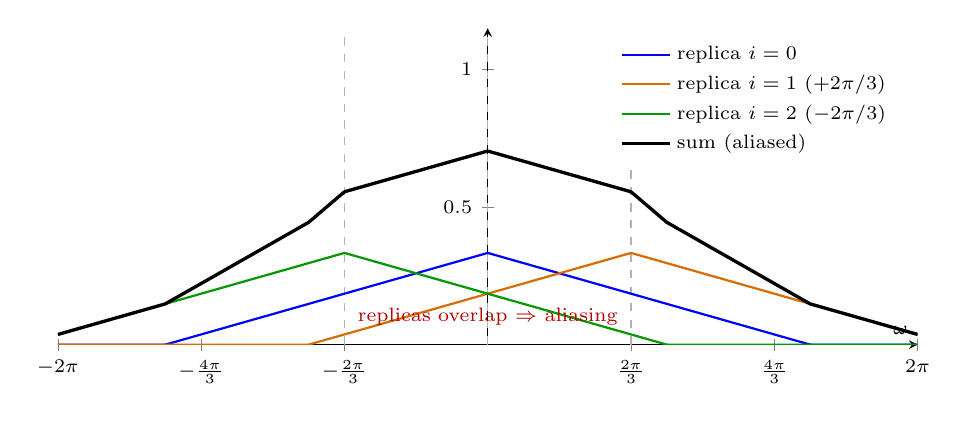
\begin{tikzpicture}
  \begin{axis}[
    width=12.5cm,
    height=5.6cm,
    axis lines=middle,
    xmin=-6.2832, xmax=6.2832, % -2π to 2π
    ymin=0, ymax=1.15,
    xtick={-6.2832,-4.1888,-2.0944,0,2.0944,4.1888,6.2832},
    xticklabels={$-2\pi$,$-\tfrac{4\pi}{3}$,$-\tfrac{2\pi}{3}$,$0$,$\tfrac{2\pi}{3}$,$\tfrac{4\pi}{3}$,$2\pi$},
    xlabel={$\omega$},
    tick label style={font=\scriptsize},
    label style={font=\scriptsize},
    title style={font=\scriptsize},
    legend cell align={left},
    legend style={font=\scriptsize, draw=none, at={(0.98,0.98)}, anchor=north east}
  ]

  % Replica centers at 0 and ±2π/3
  \draw[gray!60, dashed] (axis cs:-2.0944,0) -- (axis cs:-2.0944,1.12);
  \draw[gray!60, dashed] (axis cs: 0,0)       -- (axis cs: 0,1.12);
  \draw[gray!60, dashed] (axis cs: 2.0944,0)  -- (axis cs: 2.0944,1.12);

  % Replicas (qualitative triangles), each scaled by 1/M with M=3
  % i=0 (center at 0)
  \addplot[blue, thick, domain=-2*pi:2*pi, samples=400]
    {(1/3.0) * max(0, 1 - abs(x)/(3*pi/2))};
  \addlegendentry{replica $i=0$}

  % i=1 (center at +2π/3)
  \addplot[orange!85!black, thick, domain=-2*pi:2*pi, samples=400]
    {(1/3.0) * max(0, 1 - abs(x - 2*pi/3)/(3*pi/2))};
  \addlegendentry{replica $i=1$ ($+2\pi/3$)}

  % i=2 (center at -2π/3)
  \addplot[green!60!black, thick, domain=-2*pi:2*pi, samples=400]
    {(1/3.0) * max(0, 1 - abs(x + 2*pi/3)/(3*pi/2))};
  \addlegendentry{replica $i=2$ ($-2\pi/3$)}

  % Sum of the three replicas (aliased result)
  \addplot[black, very thick, domain=-2*pi:2*pi, samples=600]
    {(1/3.0) * max(0, 1 - abs(x)/(3*pi/2))
    + (1/3.0) * max(0, 1 - abs(x - 2*pi/3)/(3*pi/2))
    + (1/3.0) * max(0, 1 - abs(x + 2*pi/3)/(3*pi/2))};
  \addlegendentry{sum (aliased)}

  \node[red!70!black, font=\scriptsize] at (axis cs:0,0.10) {replicas overlap $\Rightarrow$ aliasing};

  \end{axis}
\end{tikzpicture}
\end{center}
\end{frame}

\section{Decimation}

\begin{frame}{Decimation: Prefiltering Before Downsampling}
\small
Problem: If original bandwidth exceeds $\pi/M$, downsampling aliases.

Solution: Apply a lowpass (antialiasing) filter of cutoff $\pi/M$ before compression.

\begin{center}
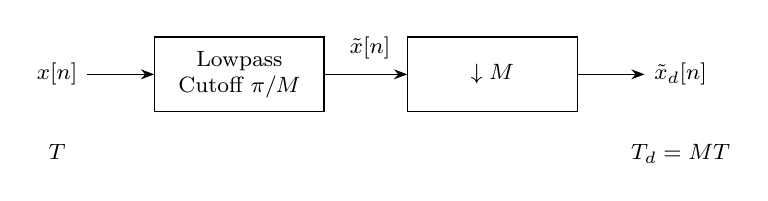
\begin{tikzpicture}[>=Stealth, node distance=0.8cm, every node/.style={font=\footnotesize}]
  \tikzset{block/.style={draw, minimum width=2.15cm, minimum height=0.95cm, align=center}}
  \node (xn) {$x[n]$};
  \node[block, right=0.85cm of xn] (lpf) {Lowpass\\Cutoff $\pi/M$};
  \node[block, right=1.05cm of lpf] (comp) {$\downarrow M$};
  \node (xdn) [right=0.85cm of comp] {$\tilde{x}_d[n]$};

  % Adjusted arrow with label placed closer to midpoint between blocks
  \draw[->] (xn.east) -- (lpf.west);
  \draw[->] (lpf.east) -- (comp.west) node[pos=0.55, above, yshift=2pt] {$\tilde{x}[n]$};
  \draw[->] (comp.east) -- (xdn.west);

  \node [below=0.5cm of xn] {$T$};
  \node [below=0.5cm of xdn] {$T_d=MT$};
\end{tikzpicture}
\end{center}

Ideal filter:
\[
\tilde{H}_d(e^{j\omega}) = \begin{cases}
1, & |\omega|\le \pi/M\\
0, & \pi/M < |\omega|\le \pi
\end{cases}
\]

After filtering, $\tilde{x}[n]$ has bandwidth $\pi/M$, so $\tilde{x}_d[n]=\tilde{x}[nM]$ is alias-free.
\end{frame}

\begin{frame}{Decimation Example: $M=3$ With Prefiltering}
\small
\begin{center}
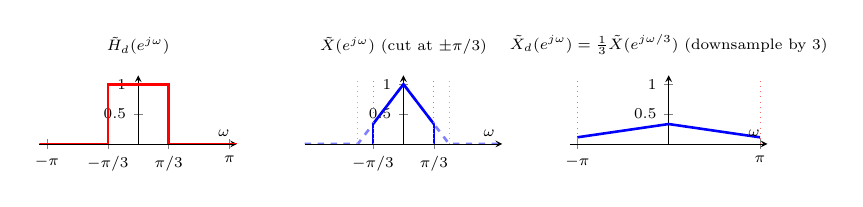
\begin{tikzpicture}[scale=0.78]
  \begin{groupplot}[
    group style={group size=3 by 1, horizontal sep=1.1cm},
    width=4.8cm,
    height=2.7cm,
    axis lines=middle,
    ymin=0, ymax=1.15,
    tick label style={font=\scriptsize},
    label style={font=\scriptsize},
    title style={font=\scriptsize}
  ]

  % 1) Ideal LPF with vertical cutoffs at ±π/3
  \nextgroupplot[
    title={$\tilde{H}_d(e^{j\omega})$},
    xmin=-3.4, xmax=3.4,
    xtick={-3.1416,-1.0472,0,1.0472,3.1416},
    xticklabels={$-\pi$,$-\pi/3$,$0$,$\pi/3$,$\pi$},
    xlabel={$\omega$}
  ]
  \addplot[red, very thick] coordinates {
    (-3.4,0) (-3.1416,0)
    (-1.0472,0) (-1.0472,1)
    ( 1.0472,1) ( 1.0472,0)
    ( 3.1416,0) ( 3.4,0)
  };

  % 2) Filtered X: original had energy to ±π/2 (triangular),
  %    after LPF it is zeroed above ±π/3.
  %    Show as a "trapezoid-like" outline: verticals at ±π/3 and a triangular top
  \nextgroupplot[
    title={$\tilde{X}(e^{j\omega})$ (cut at $\pm\pi/3$)},
    xmin=-3.4, xmax=3.4,
    xtick={-1.0472,0,1.0472},
    xticklabels={$-\pi/3$,$0$,$\pi/3$},
    xlabel={$\omega$}
  ]
  % Original (pre-filter) triangular spectrum to ±π/2 (faint, dashed for context)
  \addplot[blue!50, dashed, very thick] coordinates {(-3.4,0) (-1.5708,0) (0,1) (1.5708,0) (3.4,0)};
  % Vertical cutoffs at ±π/3 (drop to 0 outside passband)
  \addplot[blue, very thick] coordinates {(-1.0472,0) (-1.0472,0.3333)};
  \addplot[blue, very thick] coordinates {( 1.0472,0.3333) ( 1.0472,0)};
  % Triangular top within passband: value 1 at 0, value 1/3 at ±π/3
  \addplot[blue, very thick] coordinates {(-1.0472,0.3333) (0,1) (1.0472,0.3333)};
  % Guides at ±π/3 and ±π/2
  \draw[red!60, dotted] (axis cs:-1.0472,0) -- (axis cs:-1.0472,1.05);
  \draw[red!60, dotted] (axis cs: 1.0472,0) -- (axis cs: 1.0472,1.05);
  \draw[gray!60, dotted] (axis cs:-1.5708,0) -- (axis cs:-1.5708,1.05);
  \draw[gray!60, dotted] (axis cs: 1.5708,0) -- (axis cs: 1.5708,1.05);

  % 3) Downsampled by M=3: \tilde{X}_d(ω) = (1/3) \tilde{X}(ω/3)
  %    Bandwidth stretches to ±π, apex scales to 1/3, edges at ±π are 1/9.
  \nextgroupplot[
    title={$\tilde{X}_d(e^{j\omega}) = \tfrac{1}{3}\tilde{X}(e^{j\omega/3})$ (downsample by 3)},
    xmin=-3.4, xmax=3.4,
    xtick={-3.1416,0,3.1416},
    xticklabels={$-\pi$,$0$,$\pi$},
    xlabel={$\omega$}
  ]
  % Triangular top from (-π, 1/9) to (0, 1/3) to (π, 1/9)
  \addplot[blue, very thick] coordinates {(-3.1416,0.1111) (0,0.3333) (3.1416,0.1111)};
  % Optional guides
  \draw[red!60, dotted] (axis cs:-3.1416,0) -- (axis cs:-3.1416,1.05);
  \draw[red!60, dotted] (axis cs: 3.1416,0) -- (axis cs: 3.1416,1.05);
  \node[green!50!black, font=\scriptsize] at (axis cs:0,-0.25) {No aliasing};
  \end{groupplot}
\end{tikzpicture}
\end{center}

Notes:
\begin{itemize}
    \item Original $X(e^{j\omega})$ (triangular to $\pm\pi/2$) is truncated by the ideal LPF to $\pm\pi/3$, producing vertical cutoffs and a triangular top peaking at 1.
    \item Downsampling by $M=3$ yields $\tilde{X}_d(e^{j\omega})=\frac{1}{3}\tilde{X}(e^{j\omega/3})$: bandwidth expands to $\pm\pi$, apex is $1/3$.
\end{itemize}
\end{frame}

\section{Summary}

\begin{frame}{Summary}
\small
\textbf{Key Concepts}:
\begin{itemize}
    \item Resampling changes sampling rate using discrete-time operations.
    \item Downsampling by \(M\): \(x_d[n] = x[nM]\).
    \item Compressor vs. Decimator: Decimator adds antialias filter.
\end{itemize}

\textbf{Frequency-Domain Relationship}:
\[
X_d(e^{j\omega}) = \frac{1}{M}\sum_{i=0}^{M-1} X\!\left(e^{j(\omega/M - 2\pi i/M)}\right)
\]

\textbf{Aliasing Condition}:
\[
\omega_N \le \frac{\pi}{M} \quad \text{(required for alias-free direct downsampling)}
\]

If violated: prefilter to bandwidth \(\pi/M\) before rate reduction.

\end{frame}

\end{document}